\section{Auswertung}
\label{sec:Auswertung}


\subsection{Bestimmung des Sättigungsstroms $I_S$}
Die Messwerte des Anodenstroms und der Anodenspannung finden sich in Tabelle~\ref{tab:anode}. Sie sind abhängig von dem angelegten Heizstrom bzw. Heizspannung, die Werte für die jeweilige Messung finden sich in Tabelle~\ref{tab:heiz}.
Aus diesen Werten lassen sich fünf Kennlinien der Hochvakuumdiode (hier Diode 2) erstellen, siehe Abbildung~\ref{fig:kennlinie}. Aus diesen Kennlinien kann der jeweilige Sättigungsstrom $I_S$ abgelesen werden - er ist durch die cyanfarbenen Linien im Plot gekennzeichnet. Die ermittelten Werte für $I_S$ finden sich in Tabelle~\ref{tab:satt}.

\begin{figure}[H]
  \centering
  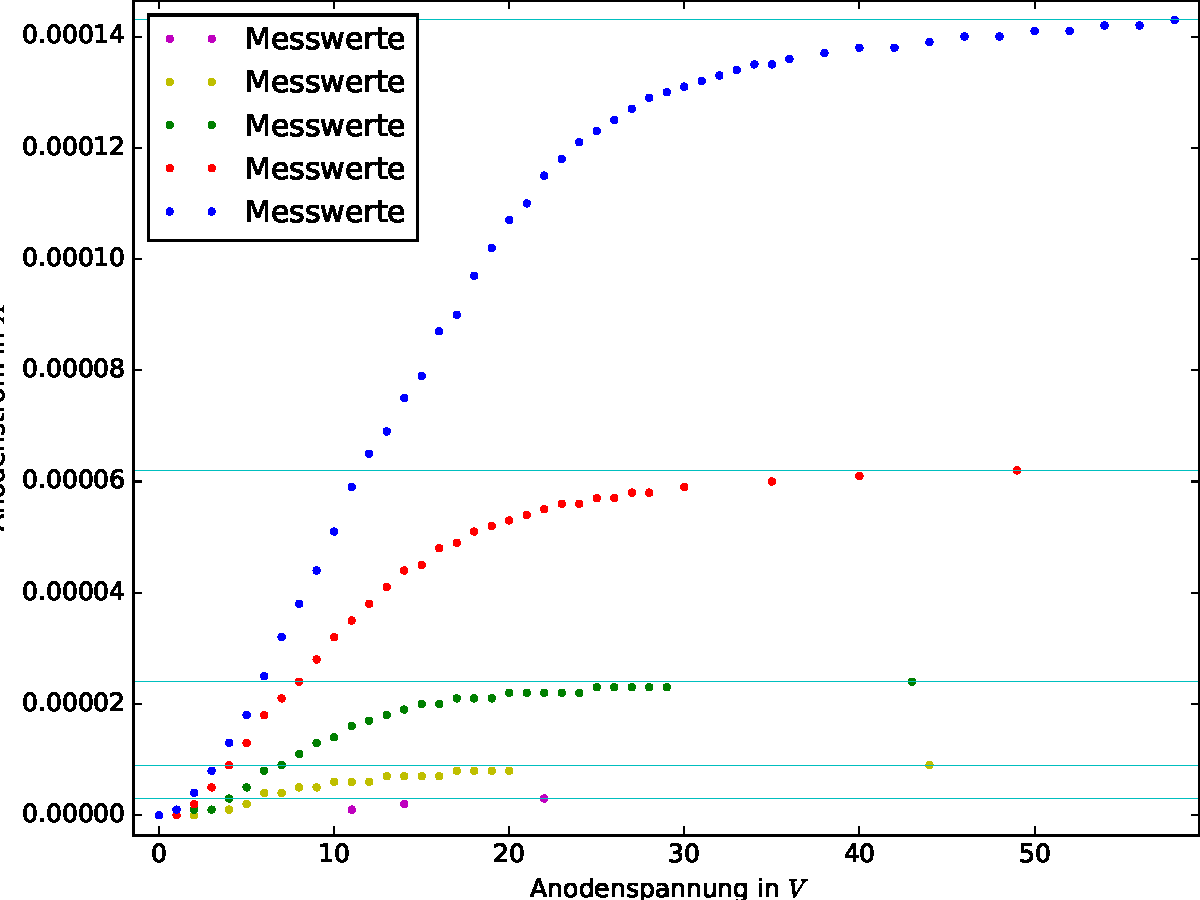
\includegraphics[width=0.6\textheight]{../plots/anode1.pdf}
  \caption{Die Kennlinien aus den Messungen 1 (blau), 2 (rot), 3 (grün), 4 (gelb) und 5 (magenta). Der jeweilige Sättigungsstrom ist durch eine cyanfarbene Linie gekennzeichnet. }
\label{fig:kennlinie}
\end{figure}

\begin{table}
  \centering
  \caption{Heizstrom und -spannung für die Messungen 1 bis 5.}
\label{tab:heiz}
  \sisetup{table-format=1.0}
  \begin{tabular}{
      S[table-format=1]
      S[table-format=7.1]
      @{${}\pm{}$}
      S[table-format=1.1]
      S[table-format=1.1]
      }
      \toprule
      \multicolumn{1}{c}{$\text{Messungsnummer}$} & \multicolumn{2}{c}{$\text{Heizspannung in $\si{\volt}$}$} & \multicolumn{1}{c}{$\text{Heizstrom in $\si{\ampere}$}$} \\
      \midrule
      \primitiveinput{../tex-data/heiz.tex}
      \bottomrule
  \end{tabular}
\end{table}


 \begin{table}
   \centering
   \caption{Anodenspannung $U_A$ und Anodenstrom $I_A$ für die Messung 1 bis 5 bei unterschiedlichem Heizstrom und Heizspannung.}
 \label{tab:anode}
   \begin{adjustbox}{center}
   \sisetup{table-format=1.0}
   \begin{tabular}{
       S[table-format=2]
       S[table-format=3]
       S[table-format=2]
       S[table-format=3]
       S[table-format=2]
       S[table-format=2]
       S[table-format=2]
       S[table-format=1]
       S[table-format=2]
       S[table-format=1]
       }
       \toprule
        $\text{$U_{A1}$ in $\si{\volt}$}$ & $\text{$I_{A1}$ in $\mathrm{\mu}\si{\ampere}$}$ & $\text{$U_{A2}$ in $\si{\volt}$}$ & $\text{$I_{A2}$ in $\mathrm{\mu}\si{\ampere}$}$ & $\text{$U_{A3}$ in $\si{\volt}$}$ & $\text{$I_{A3}$ in $\mathrm{\mu}\si{\ampere}$}$ & $\text{$U_{A4}$ in $\si{\volt}$}$ & $\text{$I_{A4}$ in $\mathrm{\mu}\si{\ampere}$}$ & $\text{$U_{A5}$ in $\si{\volt}$}$ & $\text{$I_{A5}$ in $\mathrm{\mu}\si{\ampere}$}$\\
       \midrule
       \primitiveinput{../tex-data/anode1.tex}
       \bottomrule
   \end{tabular}
 \end{adjustbox}
 \end{table}

 \begin{table}
   \centering
   \caption{Sättigungsstrom $I_S$ von Messung 1 bis 5.}
 \label{tab:satt}
   \sisetup{table-format=1.0}
   \begin{tabular}{
       S[table-format=1]
       S[table-format=3]
       }
       \toprule
        $\text{Messungsnummer}$ & $\text{$I_S$ in $\mathrm{\mu}\si{\ampere}$}$\\
       \midrule
       \primitiveinput{../tex-data/saturation.tex}
       \bottomrule
   \end{tabular}
 \end{table}

\subsection{Ermittlung des Langmuir-Schottkyschen Exponenten}
Die Kennlinie mit dem maximalen Heizstrom von $\SI{2.0}{\ampere}$ (Messung 1, siehe Tabelle~\ref{tab:anode}) ist am besten geeignet um den Langmuir-Schottkyschen Exponenten zu bestimmen. Der Gültigkeitsbereich ist erkennbar, wenn man die Kennlinie doppeltlogarithmisch aufträgt, da sich der Gültigkeitsbereich dort linear verhält\footnote{Die anderen Bereiche können schon dem Anlaufstrom- bzw. Sättigungsstromgebiet zugeordnet werden.}.
Das ist bei Kennlinie 1 in einem Bereich von $8 \mathrm{\mu} \si{\ampere}$ bis $120 \mathrm{\mu} \si{\ampere}$ gegeben. Um den Exponenten zu berechnen, muss zuerst Gleichung~\eqref{equ:shottky-langumir} durch Logarithmieren wie folgt linearisiert werden:
\begin{align}
  \ln{(\frac{I_A}{[A]})} = \frac{3}{2} \ln{(\frac{U_A}{[V]})} + \ln{(\frac{4}{9}\frac{\varepsilon_0}{d^2} \sqrt{\frac{2 e_0}{m_0}})} \; .
\end{align}

Nun kann mit Hilfe der \emph{curvefit}-Funktion aus \emph{python} eine lineare Ausgleichsrechnung vorgenommen werden\footnote{Alle folgenden Fits werden mit dieser Funktion durchgeführt.}, die folgende Parameter ergibt:
\begin{align}
  \ln{(\frac{I_A}{[A]})} = (1.356 \pm 0.035) \ln{(\frac{U_A}{[V]})} + (-13.079 \pm 0.083) \; .
\end{align}

Die Steigung der Geraden gibt den Langmuir-Schottkyschen Exponenten an und beträgt $(1.356 \pm 0.035)$. Die Abweichung vom Theoriewert, der $1.5$\footnote{Skript V504} beträgt, ist ca. $9.6\%$. Die Messwerte sowie der lineare Fit sind in Abbildung~\ref{fig:langmuh} zu finden.

\begin{figure}[H]
  \centering
  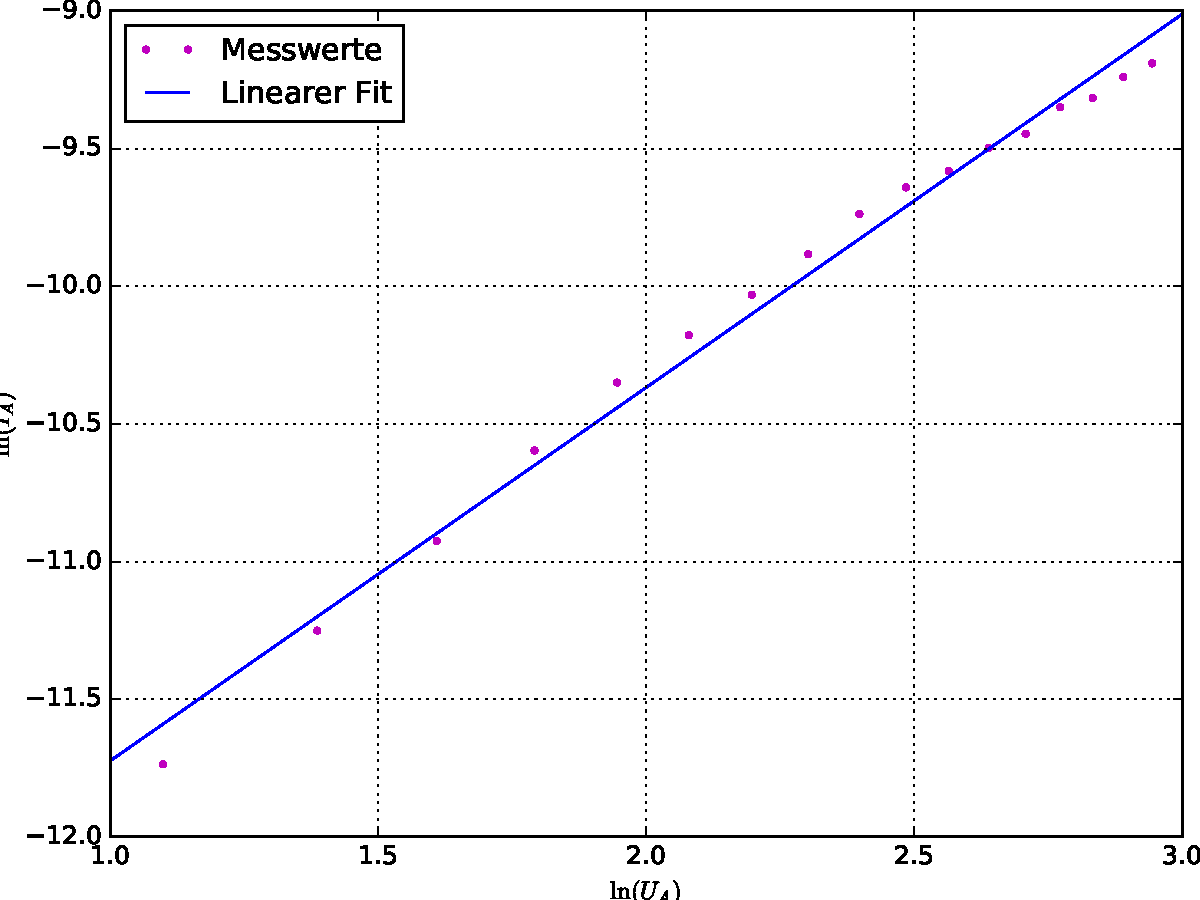
\includegraphics[width=0.6\textheight]{../plots/langmuh.pdf}
  \caption{Messwerte aus dem Gültigkeitsbereich des Raumladungsgebiets mit linearem Fit. }
\label{fig:langmuh}
\end{figure}

\subsection{Bestimmung der Kathodentemperatur}
\subsubsection{Mit Hilfe des Anlaufstromgebiets}
Das Nanoamperemeter, mit dessen Hilfe der Anlaufstrom gemessen werden soll, verändert die gemessene Spannung\footnote{Aufgrund des Spannungsabfalls am Innenwiderstand des Messgeräts.} $U_{\mathrm{Messung}}$. Aus diesem Grund muss vor der Berechnung der Kathodentemperatur eine Korrektur vorgenommen werden. Der Innenwiderstand $R$ des Geräts beträgt $\SI{1}{\mega\ohm}$. Weiterhin ist zu beachten, dass die Autoren diesen Versuchsteil an einer anderen Diode vorgenommen haben, nämlich an Gerät 1, welches einen maximalen Heizstrom von $\SI{2.5}{\ampere}$ zulässt. Die reale Spannung $U_{\mathrm{real}}$ ergibt sich aus
\begin{align}
  U_{\mathrm{real}} = U_{\mathrm{Messung}} - I_A R \; .
\end{align}
Die Messdaten sowie die korrigierten Werte finden sich in Tabelle~\ref{tab:real}.

\begin{table}
  \centering
  \caption{Stromstärke, Spannung und korrigierte Spannung im Anlaufstromgebiet.}
\label{tab:real}
  \sisetup{table-format=1.0}
  \begin{tabular}{
      S[table-format=2.2]
      S[table-format=2.2]
      S[table-format=1.4]
      }
      \toprule
       $\text{$I_A$ in $\si{\nano\ampere}$}$ & $\text{$U_{\mathrm{Messung}}$ in $\si{\volt}$}$ & $\text{$U_{\mathrm{real}}$ in $\si{\volt}$}$\\
      \midrule
      \primitiveinput{../tex-data/Ureal.tex}
      \bottomrule
  \end{tabular}
\end{table}

Zur Bestimmung der Kathodentemperatur wird Gleichung~\eqref{equ:anlauf} zu
\begin{align}
  \ln{(\frac{I_A}{[A]})} = \underbrace{- \frac{e_0}{k_B T}}_{m} \cdot U_{\mathrm{real}} + \underbrace{\ln{(\mathrm{const})}}_{b}
\end{align}
linearisiert. Mit Hilfe einer linearen Ausgleichsrechnung kann nun $m$ bestimmt und zu $T$ umgeformt werden:
\begin{align}
  \ln{(\frac{I_A}{[A]})} &= \underbrace{(4.728 \pm 0.041)}_{m} \cdot \frac{U_{\mathrm{real}}}{[V]} + (-17.984 \pm -0.023) \\
  \Leftrightarrow T &= \frac{e_0}{k_B m} \; .
\end{align}

Die Ausgleichsgerade findet sich zusammen mit den Messwerten in Abbildung~\ref{fig:T}
Mit der Elementarladung $e_0~=~1.602176~\cdot~10^{-19}~\si{\coulomb}$ und der Boltzmannkonstante $k_B~=~1.38064852~\cdot~10^{23}~\si{\joule\per\kelvin}$ ergibt sich die Kathodentemperatur zu
\begin{align}
  T = (2454 \pm 21) \si{\kelvin} \; .
\end{align}

\begin{figure}[H]
  \centering
  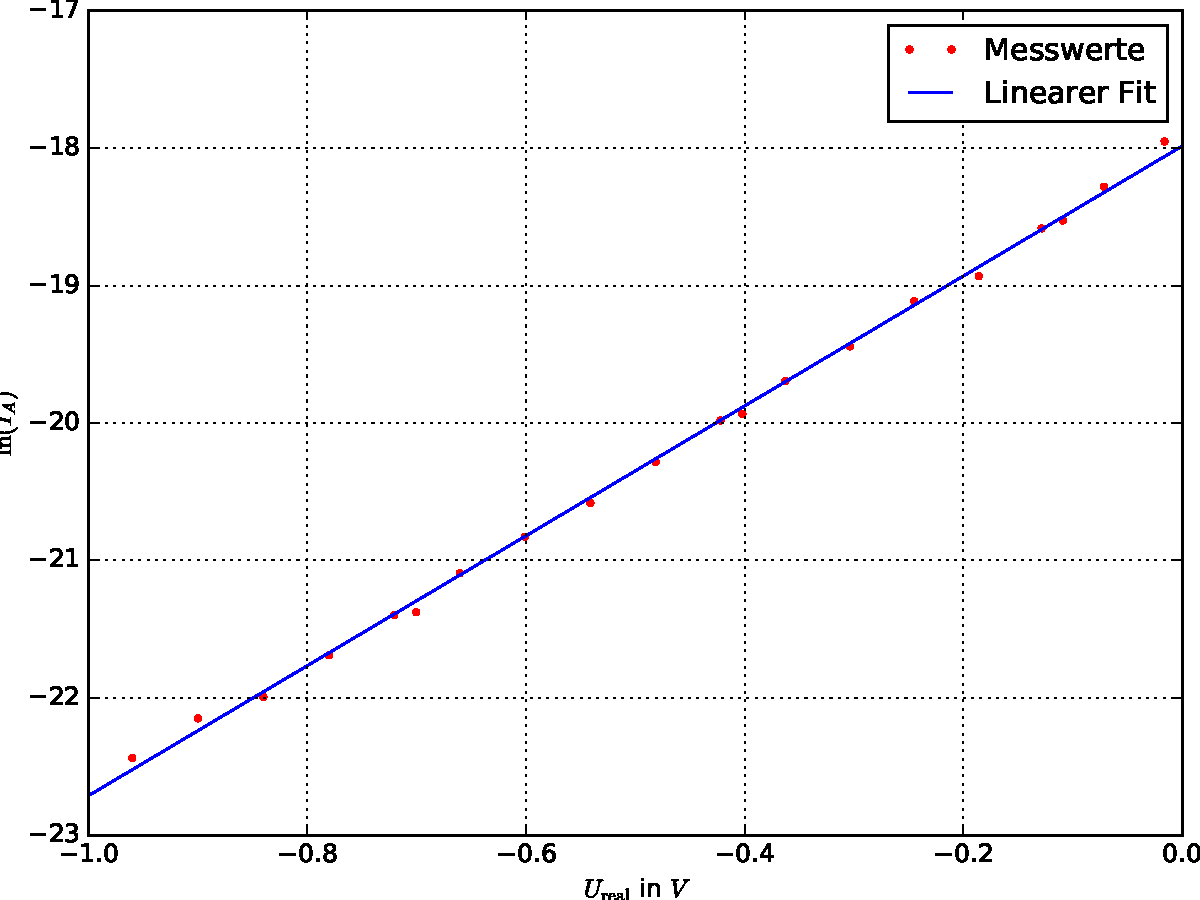
\includegraphics[width=0.6\textheight]{../plots/current.pdf}
  \caption{Messwerte des Anlaufstromgebiets mit linearem Fit. }
\label{fig:T}
\end{figure}

\subsubsection{Mit Hilfe der Kennlinien}
Aus den Kennlinien kann die Kathodentemperatur $T$ über die Leistungsbilanz des Heizstromfadens berechnet werden. Für die zugeführte Leistung $N_{\mathrm{zu}}$ der Kathode gilt:
\begin{align}
  N_{\mathrm{zu}} &= U_{\mathrm{Heiz}} \cdot I_{\mathrm{Heiz}} \\
  &= f \eta \sigma T^4 + N_{\mathrm{WL}} \\
    \Leftrightarrow T &= \sqrt[4]{\frac{U_{\mathrm{Heiz}} \cdot I_{\mathrm{Heiz}} - N_{\mathrm{WL}}}{f \eta \sigma}} \; .
\end{align}

Die Wertepaare für die Heizspannung und den Heizstrom befinden sich in Tabelle~\ref{tab:heiz}. Die emittierende Kathodenfläche beträgt $f = \SI{0.35}{\square\centi\m}$ für Diode~2, die Stefan-Boltzmannsche Strahlungskonstante $\sigma = \SI{5.7e-12}{\watt\centi\m{^{-2}}\kelvin{^{-4}}}$ und der Emissionsgrad der Oberfläche $\eta = 0.28$. Die Wärmeleitung wird mit $N_{\mathrm{WL}} = \SI{0.95}{\watt}$ abgeschätzt.
Die Kathodentemperaturen für jede gemessene Kennlinie findet sich in Tabelle~\ref{tab:Temp}.

\begin{table}
  \centering
  \caption{Kathodentemperatur für die Messungen 1 bis 5.}
\label{tab:Temp}
  \sisetup{table-format=1.0}
  \begin{tabular}{
      S[table-format=1]
      S[table-format=4]
      @{${}\pm{}$}
      S[table-format=2]
      }
      \toprule
      \multicolumn{1}{c}{$\text{Messungsnummer}$} & \multicolumn{2}{c}{$\text{$T_{\mathrm{Kath}}$ in $\si{\kelvin}$}$} \\
      \midrule
      \primitiveinput{../tex-data/temp.tex}
      \bottomrule
  \end{tabular}
\end{table}

\subsection{Bestimmung der Austrittsarbeit von Wolfram}
Die Richardson Gleichung~\eqref{equ:richardson} kann nach der Austrittsarbeit~$e_0\Phi$ umgestellt werden:
\begin{align}
  e_0\Phi = k_B T_{\mathrm{Kath}} \ln{(\frac{4 \pi e_0 m_0 f k_B^2}{h^3 I_S} \cdot T_{\mathrm{Kath}}^2 )} \; .
\end{align}
Mit dem Planckschen Wirkungsquantum $h = \SI{6.626070040e-34}{\joule\second}$ und der Elektronenmasse $m_0 = \SI{9.10938356e-31}{\kg}$ ergibt sich die gemittelte Austrittsarbeit von Wolfram zu $(7.334 \pm 0.103)~e\si{\volt}$. Dieser Wert weicht vom Literaturwert ($4.5~e\si{\volt}$) um ca. $63\%$ ab.

\begin{table}
  \centering
  \caption{Austrittsarbeit von Wolfram für die Messungen 1 bis 5.}
\label{tab:arbeit}
  \sisetup{table-format=1.0}
  \begin{tabular}{
      S[table-format=1]
      S[table-format=1.3]
      @{${}\pm{}$}
      S[table-format=1.3]
      }
      \toprule
      \multicolumn{1}{c}{$\text{Messungsnummer}$} & \multicolumn{2}{c}{$\text{$e_0\Phi$ in $e\si{\volt}$}$} \\
      \midrule
      \primitiveinput{../tex-data/arbeit.tex}
      \bottomrule
  \end{tabular}
\end{table}


% \begin{table}
%   \centering
%   \caption{Geschwindigkeiten der Öltröpfchen mit zugehöriger angelegter Ladung. Eine nicht vorliegende Messung ist durch den Wert 0 gekennzeichnet.}
% \label{tab:v}
%   \sisetup{table-format=1.0}
%   \begin{tabular}{
%       S[table-format=3]
%       S[table-format=1.2]
%       S[table-format=2.2]
%       S[table-format=2.2]
%       }
%       \toprule
%        $\text{Spannung in V}$ & $\text{$v_0$ in $10^{-5} \si{\m\per\second}$}$ & $\text{$v_{\mathrm{ab}}$ in $10^{-5} \si{\m\per\second}$}$
%        & $\text{$v_{\mathrm{auf}}$ in $10^{-5} \si{\m\per\second}$}$\\
%       \midrule
%       \primitiveinput{../tex-data/v.tex}
%       \bottomrule
%   \end{tabular}
% \end{table}

%\begin{figure}[H]
%  \centering
%  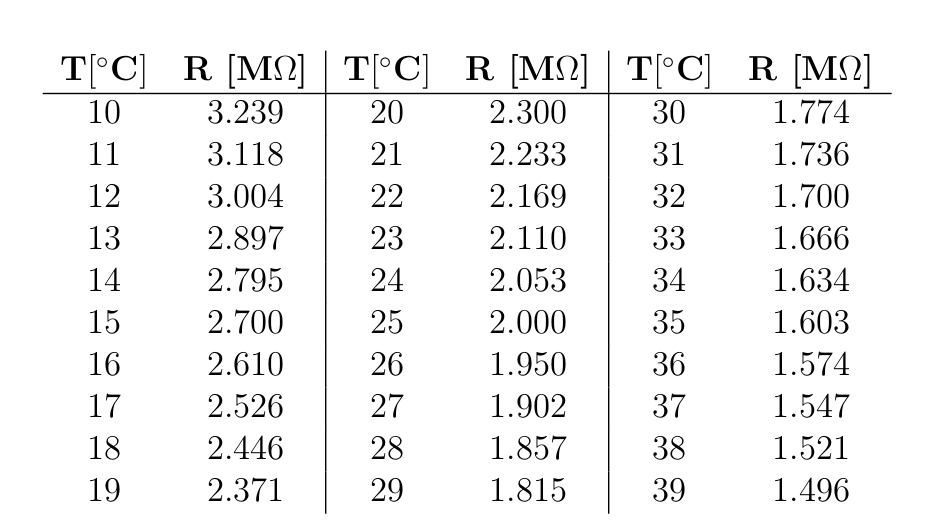
\includegraphics[width=0.4\textheight]{../figures/tab.png}
%  \caption{Thermistor-Widerstandstabelle. [Skript V503]}
%\label{fig:T}
%\end{figure}

%the end
